\subsection{Example: Inverted slider-crank Mechanism}
\begin{frame}{Normal Approach}
\begin{block}{Example 1: Inverted slider-crank Mechanism}
	\begin{table}
		\begin{minipage}{0.5\linewidth}
			\begin{tabular}{l|l}
				      & $l_{AC} = 0.15m$\\
				      & $l_{BC} = 0.2m$\\
				      & $l_{AD} = 0.35m$\\
				Given & $\theta_1=60^\circ$ \\
					  & $\vb{\omega}{1} = \pi\kh $ $(rad/s)$\\
					  & $\vb{\alpha}{1} = \vb{0}{} $ $(rad/s^2)$ \\\hline
				Find  & $\vb{v}{B_3}$, $\vb{v}{D}$, $\vb{a}{B_3}$, $\vb{a}{D}$,\\
				&$\vb{\omega}{2}$, $\vb{\alpha}{2}$\\
			\end{tabular}
		\end{minipage}\hfill
		\begin{minipage}{0.5\linewidth}
			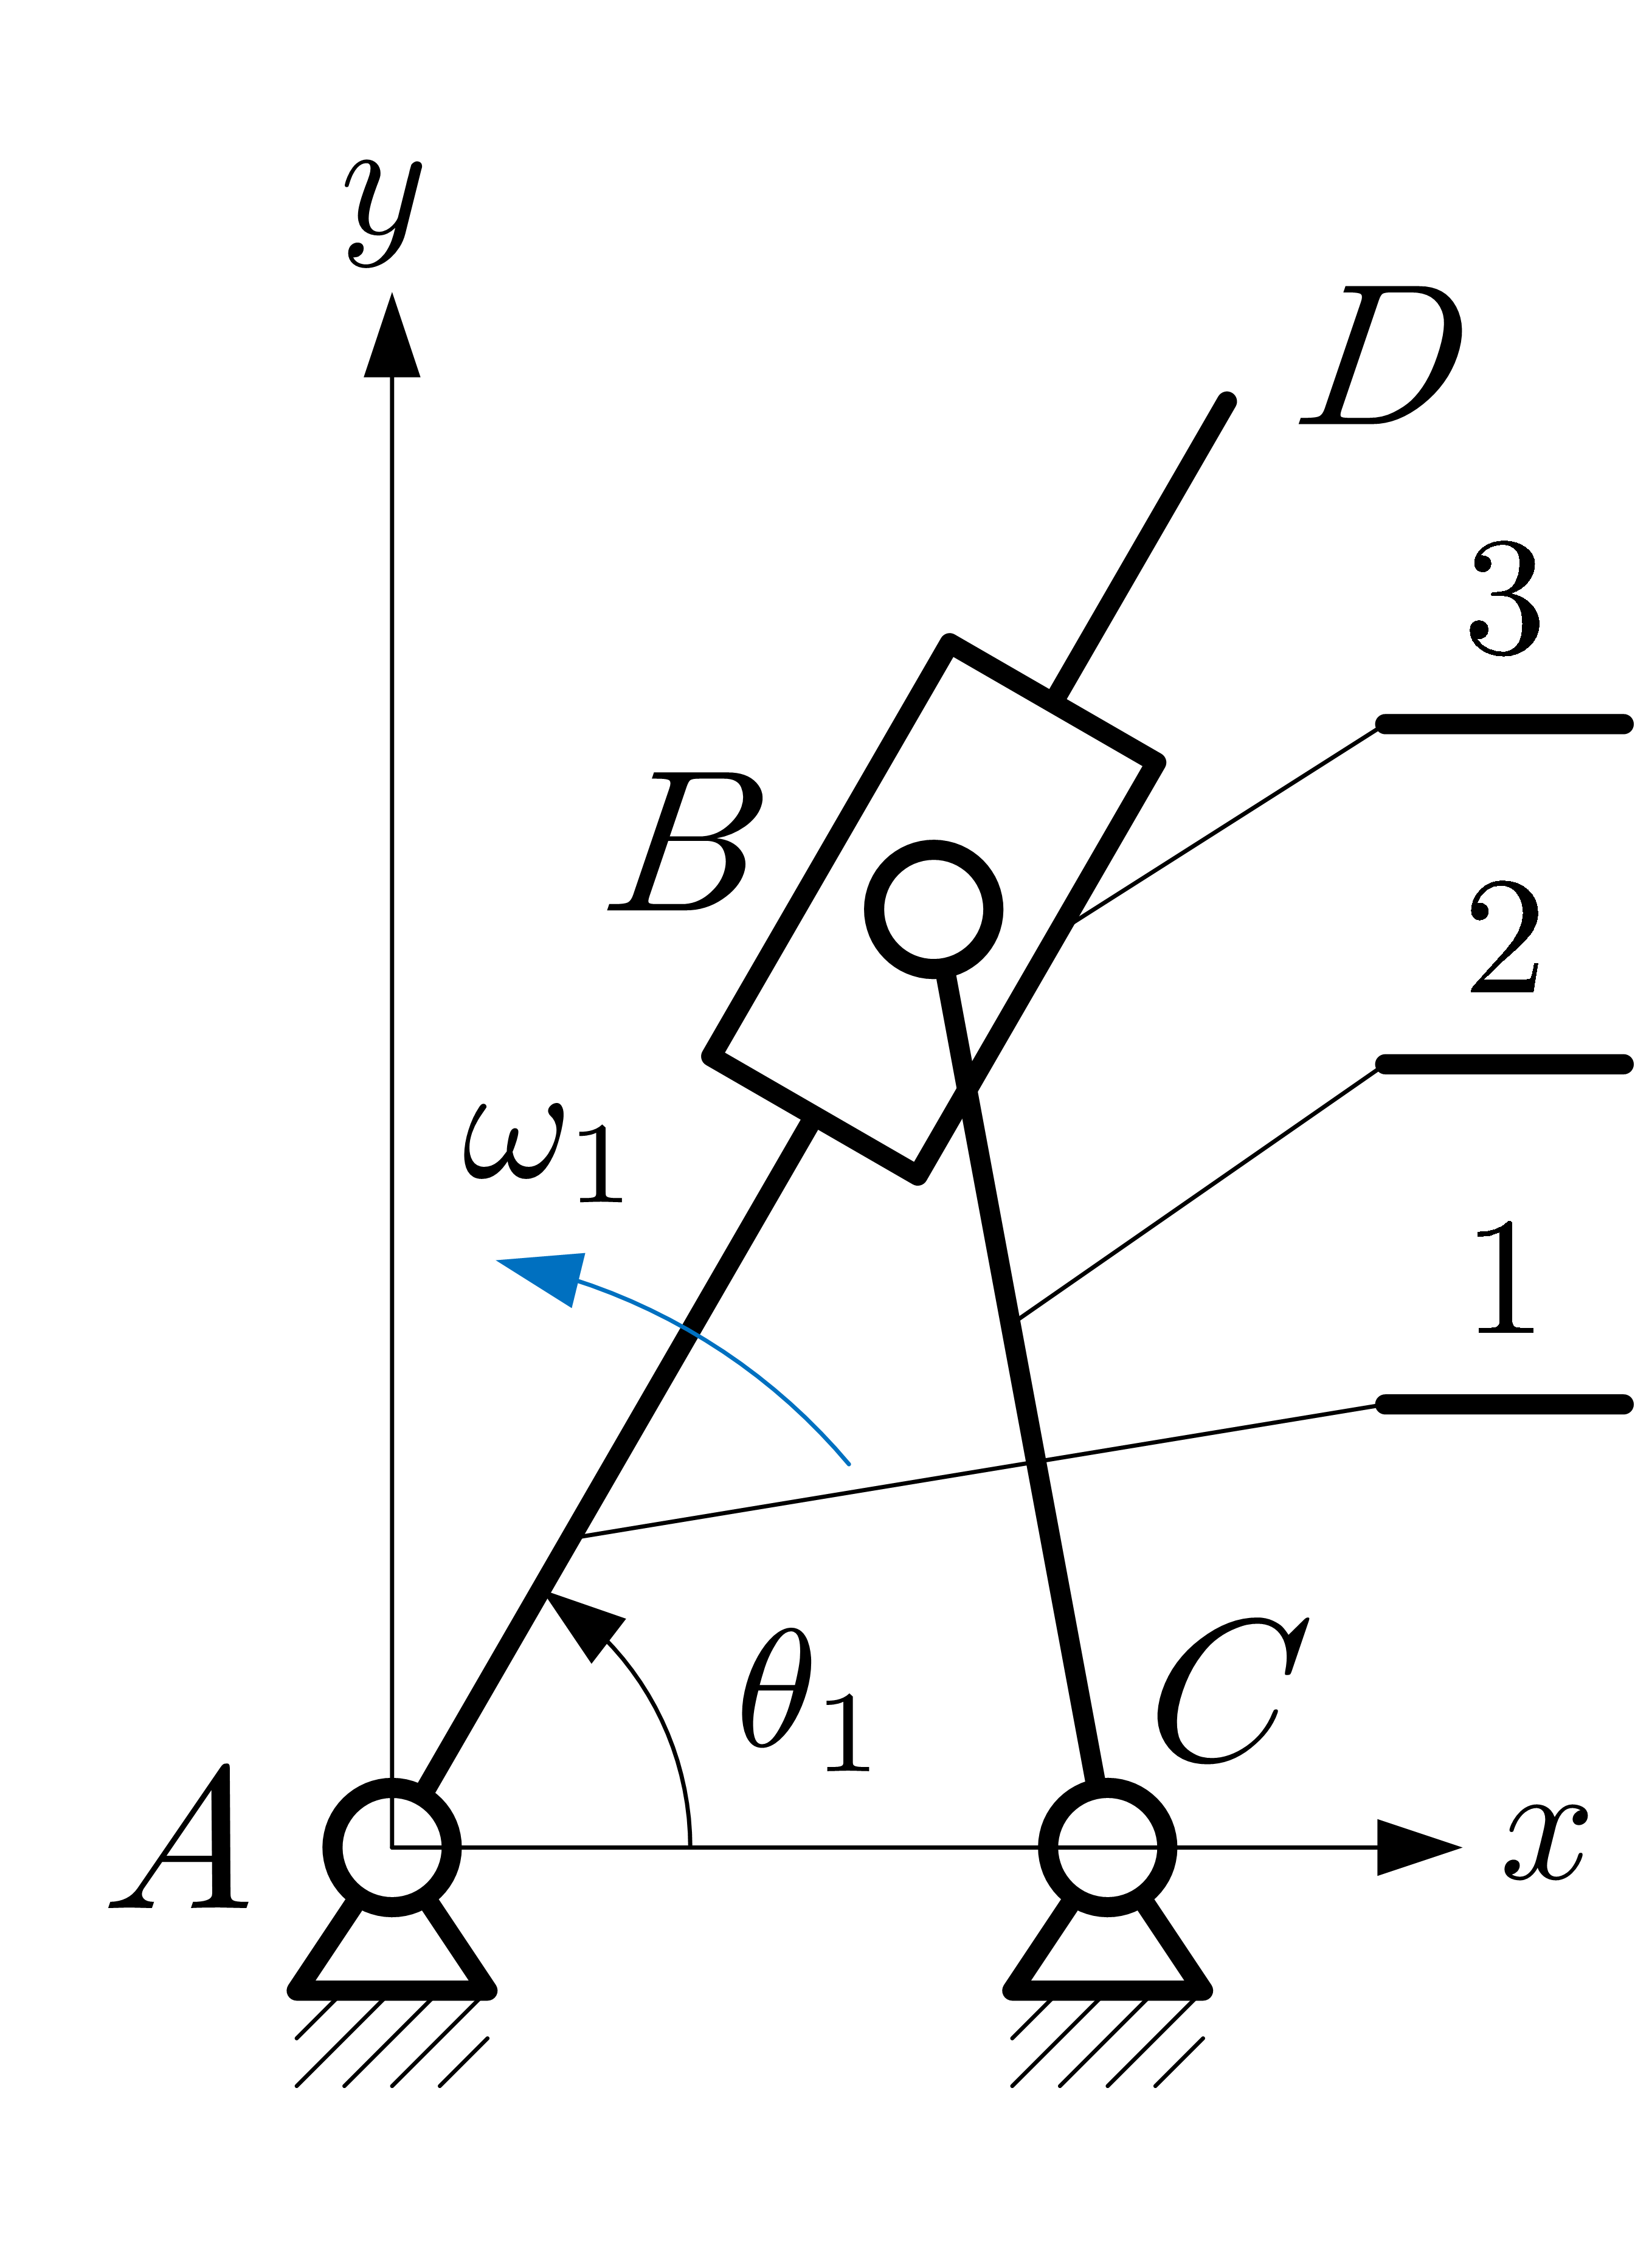
\includegraphics[width =30mm]{images/Inverted-R-RRT.png}
		\end{minipage}
	\end{table}
\end{block}
\emph{Solution}\vskip2.5mm
Using position analysis / MATLAB,\\
$\Rightarrow \vb{r}{B} = 0.1135\ih + 0.1966\jh\text{ }(m)$, $\vb{r}{C} = 0.15\ih\text{ }(m)$

\end{frame}

\begin{frame}
$\vb{r}{BC} = \vb{r}{B} - \vb{r}{C} = -0.0365\ih + 0.1966\jh\text{ }(m)$
\begin{itemize}
\item Find $\vb{v}{B_1}$\vskip1.25mm
$\vb{v}{B_1} = \vb{\omega}{1}\times\vb{r}{B} = -0.6178\ih + 0.3567\jh\text{ }(m)$\vskip2.5mm
\item Find $\vb{v}{B_2B_1} = v_{Bx}\ih + v_{By}\jh$, $\vb{\omega}{3} = \vb{\omega}{2} = \omega_{3z}\kh$\vskip1.25mm
$\begin{cases}
\vb{v}{B_2} = \vb{v}{B_1} + \vb{v}{B_2B_1} \Leftrightarrow \vb{\omega}{3}\times\vb{r}{BC} = \vb{v}{B_1} + \vb{v}{B_2B_1}\\
(\vb{r}{B}\times\ih)\times\vb{r}{B}\cdot\vb{v}{B_2}=0
\end{cases}$\vskip2.5mm
Projecting onto $x,y$-axes, we obtain the solution:\vskip1.25mm
$\Rightarrow\begin{cases}
v_{Bx} = -0.3047\text{ }(m/s)\\v_{By} = -0.5277\text{ }(m/s)\\\omega_{3z} = 4.691\text{ }(rad/s)
\end{cases}$\\$\Rightarrow\begin{cases}
\vb{v}{B_2B_1} = -0.3047\ih - 0.5277\jh\text{ }(m/s)\\ \vb{\omega}{3} = \vb{\omega}{2} = 4.691\kh\text{ }(rad/s)
\end{cases}$\\
\end{itemize}
\end{frame}

\begin{frame}
	\begin{itemize}
		\item Find $\vb{v}{B} = \vb{v}{B_2}$, $\vb{v}{D}$\vskip1.25mm
		$\vb{v}{B} = \vb{v}{B_2} = \vb{\omega}{3}\times\vb{r}{BC} = -0.9225\ih - 0.1711\jh\text{ } (m/s)$\\
		$\vb{v}{D} = \vb{\omega}{1}\times\vb{r}{BC} = -0.9522\ih + 0.5498\jh\text{ } (m/s)$
	\end{itemize}
\end{frame}

\begin{frame}
\begin{itemize}
\item Find $\vb{a}{B_1}$, $\vb{a}{B_2}^{\bm{n}}$, $\vb{a}{B_2B_1}^{\bm{c}}$\vskip1.25mm
$\vb{a}{B_1} = \vb{\alpha}{1}\times \vb{r}{B} - \vb{\omega}{1}^2\vb{r}{B}=-1.1205\ih - 1.9408\jh \text{ }(m/s^2)$\\
$\vb{a}{B_2}^{\bm{n}} = -\vb{\omega}{3}^2\vb{r}{BC}=0.8024\ih-4.3274\jh\text{ }(m/s^2)$\\
$\vb{a}{B_2B_1}^{\bm{c}} = 2\vb{\omega}{1}\times\vb{v}{B_2B_1} = 3.3159\ih - 1.9144\jh\text{ }(m/s^2)$\vskip2.5mm
\item Find $\vb{a}{B_2B_1}^{\bm{r}} = a_{Bx}\ih + a_{By}\jh$, $\vb{\alpha}{3} = \vb{\alpha}{2} = \alpha_{3z}\kh$\vskip1.25mm
$\begin{cases}
\vb{a}{B_2} = \vb{a}{B_1} + \vb{a}{B_2B_1}\\ \Leftrightarrow \vb{\alpha}{3}\times\vb{r}{BC} + \vb{a}{B_2}^{\bm{n}} = \vb{a}{B_1} + \vb{a}{B_2B_1}^{\bm{c}} + \vb{a}{B_2B_1}^{\bm{r}}\\
(\vb{r}{B}\times\ih)\times\vb{r}{B}\cdot\vb{a}{B_2B_1}^{\bm{r}}=0
\end{cases}$

\end{itemize}
\end{frame}
\begin{frame}
	\begin{itemize}
		\item[]Projecting onto $x,y$-axes, we obtain the solution:\vskip1.25mm
		$\Rightarrow\begin{cases}
		a_{Bx} = -0.1382\text{ }(m/s^2)\\a_{By} = -0.2394\text{ }(m/s^2)\\\alpha_{3z}=-6.3802\text{ }(rad/s^2)
		\end{cases}$\\
		$\Rightarrow\begin{cases}
		\vb{a}{B_2B_1}^{\bm r} = -0.1382\ih - 0.2394\jh\text{ }(m/s^2)\\\vb{\alpha}{3} = \vb{\alpha}{2}=-6.3802\kh\text{ }(rad/s^2)
		\end{cases}$\vskip2.5mm
		\item Find $\vb{a}{B} = \vb{a}{B_2}$, $\vb{a}{D}$\vskip1.25mm
		$\vb{a}{B} = \vb{a}{B_2} = \vb{\alpha}{3}\times\vb{r}{BC} - \vb{\omega}{3}^2\vb{r}{BC} = 2.0571\ih - 4.0947\jh\text{ } (m/s^2)$\\
		$\vb{a}{D} = \vb{\alpha}{1}\times \vb{r}{D} - \vb{\omega}{1}^2\vb{r}{D} = -1.7272\ih - 2.9916\jh\text{ } (m/s^2)$
	\end{itemize}
\end{frame}

\begin{frame}{MATLAB R2019a code}
\lstinputlisting[style=Matlab-editor, basicstyle = \mlttfamily]{codes/i-s-c_v.m}
\end{frame}
\begin{frame}{MATLAB R2019a code}
\lstinputlisting[style=Matlab-editor, basicstyle = \mlttfamily]{codes/i-s-c_a.m}
\end{frame}
\begin{frame}{MATLAB R2019a code}
\lstinputlisting[style=Matlab-editor, basicstyle = \mlttfamily]{codes/i-s-c_a_2.m}
\end{frame}


\begin{frame}{Derivative Method}
Let $\theta_1 = \theta(t)$ be a function of time $t$. We perform position analysis to find $\vb{r}{B}(\theta(t))$ and $\vb{r}{D}(\theta(t))$. Using MATLAB, we find out that:\vskip1.25mm
\hskip10mm$\displaystyle \vb{r}{B}(\theta(t)) =  \frac{3\cos{\theta(t)}+\sqrt{9\cos{\theta(t)}^2+7}}{20}(\cos{\theta(t)}\ih + \sin{\theta(t)}\jh)$\vskip2.5mm
\hskip10mm$\displaystyle \vb{r}{D}(\theta(t)) = \frac{7}{20}\cos{\theta(t)}\ih + \frac{7}{20}\sin{\theta(t)}\jh$\vskip2.5mm
Using the results above to obtain the angle  $\theta_3(\theta(t))$ of link 3:
\[
\theta_3(\theta(t)) = \arctan{\left(\cot{\theta(t)}\frac{3\cos{\theta(t)}+\sqrt{9\cos{\theta(t)}^2+7}}{\sqrt{9\cos{\theta(t)}^2+7}+3\cos{\theta(t)}^2-3}\right)}
\]
\end{frame}

\begin{frame}
Then, find velocities and accelerations by taking first and second derivative of $\vb{r}{B}$, $\vb{r}{D}$, $\theta_2$, respectively:
\[\begin{cases}
\displaystyle \vb{v}{B_2}(\theta(t)) = \xvec[.]{\bm{r}}_{\bm{B}}\\\displaystyle \vb{v}{D}(\theta(t)) = \xvec[.]{\bm{r}}_{\bm{D}}\\\displaystyle \vb{\omega}{3}(\theta(t)) = \dot{\theta_3}\kh
\end{cases}, \begin{cases}
\displaystyle \vb{a}{B_2}(\theta(t)) = \xvec[:]{\bm{r}}_{\bm{B}}\\\displaystyle \vb{a}{D}(\theta(t)) = \xvec[:]{\bm{r}}_{\bm{D}}\\\displaystyle \vb{\alpha}{3}(\theta(t)) = \ddot{\theta_3}\kh
\end{cases}\]
Let $\theta(t)=60^\circ$, we obtain the final results.
\end{frame}
\begin{frame}{MATLAB R2019a code}
\lstinputlisting[style=Matlab-editor, basicstyle = \mlttfamily]{codes/i-s-c_p_d.m}
\end{frame}
\begin{frame}{MATLAB R2019a code}
\lstinputlisting[style=Matlab-editor, basicstyle = \mlttfamily]{codes/i-s-c_v_a_d.m}
\end{frame}
\begin{frame}{Independent Contour Method}
Using the solution above,\vskip1.25mm
$\vb{r}{B} = 0.1135\ih + 0.1966\jh\text{ }(m)$, $\vb{r}{C} = 0.15\ih\text{ }(m)$ \\
$\vb{r}{BC}= -0.0365\ih + 0.1966\jh \text{ $(m)$}$, $ \vb{a}{B_1} = -1.1205\ih - 1.9408\jh \text{ $(m/s^2)$}$\vskip2.5mm
Applying velocity formulas to find $\vb{v}{12} = v_{12x}\ih + v_{12y}\jh$, $\vb{\omega}{23} = \omega_{23z}\kh$, $\vb{\omega}{30} = \omega_{30z}\kh$:\vskip1.25mm
$\hskip5mm\begin{cases}
\vb{\omega}{01} + \vb{\omega}{23} + \vb{\omega}{30} = \vb{0}{}\\
\vb{r}{B}\times\vb{\omega}{23}+\vb{r}{C}\times\vb{\omega}{30}+\vb{v}{12}= \vb{0}{}\\
(\vb{r}{B}\times\ih)\times\vb{r}{B}\cdot\vb{v}{12}=0
\end{cases}$\vskip2.5mm
Solving the system of equations by projecting onto $x,y$-axes, we obtain:\vskip1.25mm
$\vb{\omega}{23} = 1.5494\kh\text{ }(rad/s)$, $\vb{\omega}{30} = -4.691\kh\text{ }(rad/s)$,\\
$\vb{v}{12} = -0.3047\ih - 0.5277\jh\text{ }(m/s)$\vskip2.5mm
The results is consistent with the 2 previous methods.
\end{frame}

\begin{frame}
Again, using acceleration formulas $\vb{a}{12} = a_{12x}\ih + a_{12y}\jh$, $\vb{\alpha}{23} = \alpha_{23z}\kh$, $\vb{\alpha}{30} = \alpha_{30z}\kh$:\vskip1.25mm
\hskip5mm$\begin{cases}
\vb{\alpha}{01} + \vb{\alpha}{23} + \vb{\alpha}{30} = \vb{0}{}\\
\vb{r}{B}\times\vb{\alpha}{23} + \vb{r}{C}\times\vb{\alpha}{30} + \vb{a}{12} - \vb{\omega}{1}^2\vb{r}{B} - \vb{\omega}{3}^2\vb{r}{CB} = \vb{0}{}\\
(\vb{r}{B}\times\ih)\times\vb{r}{B}\cdot\vb{a}{12}=0
\end{cases}$\vskip2.5mm
Solving the system of equations by projecting onto $x,y$-axes, we obtain:\vskip1.25mm $\vb{\alpha}{23} = -6.3802\kh\text{ }(rad/s^2)$, $\vb{\alpha}{30} = 6.3802\kh\text{ }(rad/s^2)$,\\
$\vb{a}{12} = -0.1382\ih - 0.2394\jh\text{ }(m/s^2)$\vskip2.5mm
The results is consistent with the 2 previous methods.
\end{frame}


\begin{frame}{MATLAB R2019a code}
\lstinputlisting[style=Matlab-editor, basicstyle= \mlttfamily]{codes/i-s-c_v_i.m}
\end{frame}
\begin{frame}{MATLAB R2019a code}
\lstinputlisting[style=Matlab-editor, basicstyle= \mlttfamily]{codes/i-s-c_v_i_2.m}
\end{frame}
\begin{frame}{MATLAB R2019a code}
\lstinputlisting[style=Matlab-editor, basicstyle= \mlttfamily]{codes/i-s-c_a_i.m}
\end{frame}
\begin{frame}{MATLAB R2019a code}
\lstinputlisting[style=Matlab-editor, basicstyle= \mlttfamily]{codes/i-s-c_a_i_2.m}
\end{frame}
\begin{frame}{Velocity - Acceleration plotting}
\lstinputlisting[style=Matlab-editor, basicstyle=\mlttfamily]{codes/i-s-c_v_a_plotting.m}
\end{frame}
\begin{frame}{Output figures}
\begin{table}
\begin{minipage}{0.5\linewidth}
	\begin{figure}
		\centering
		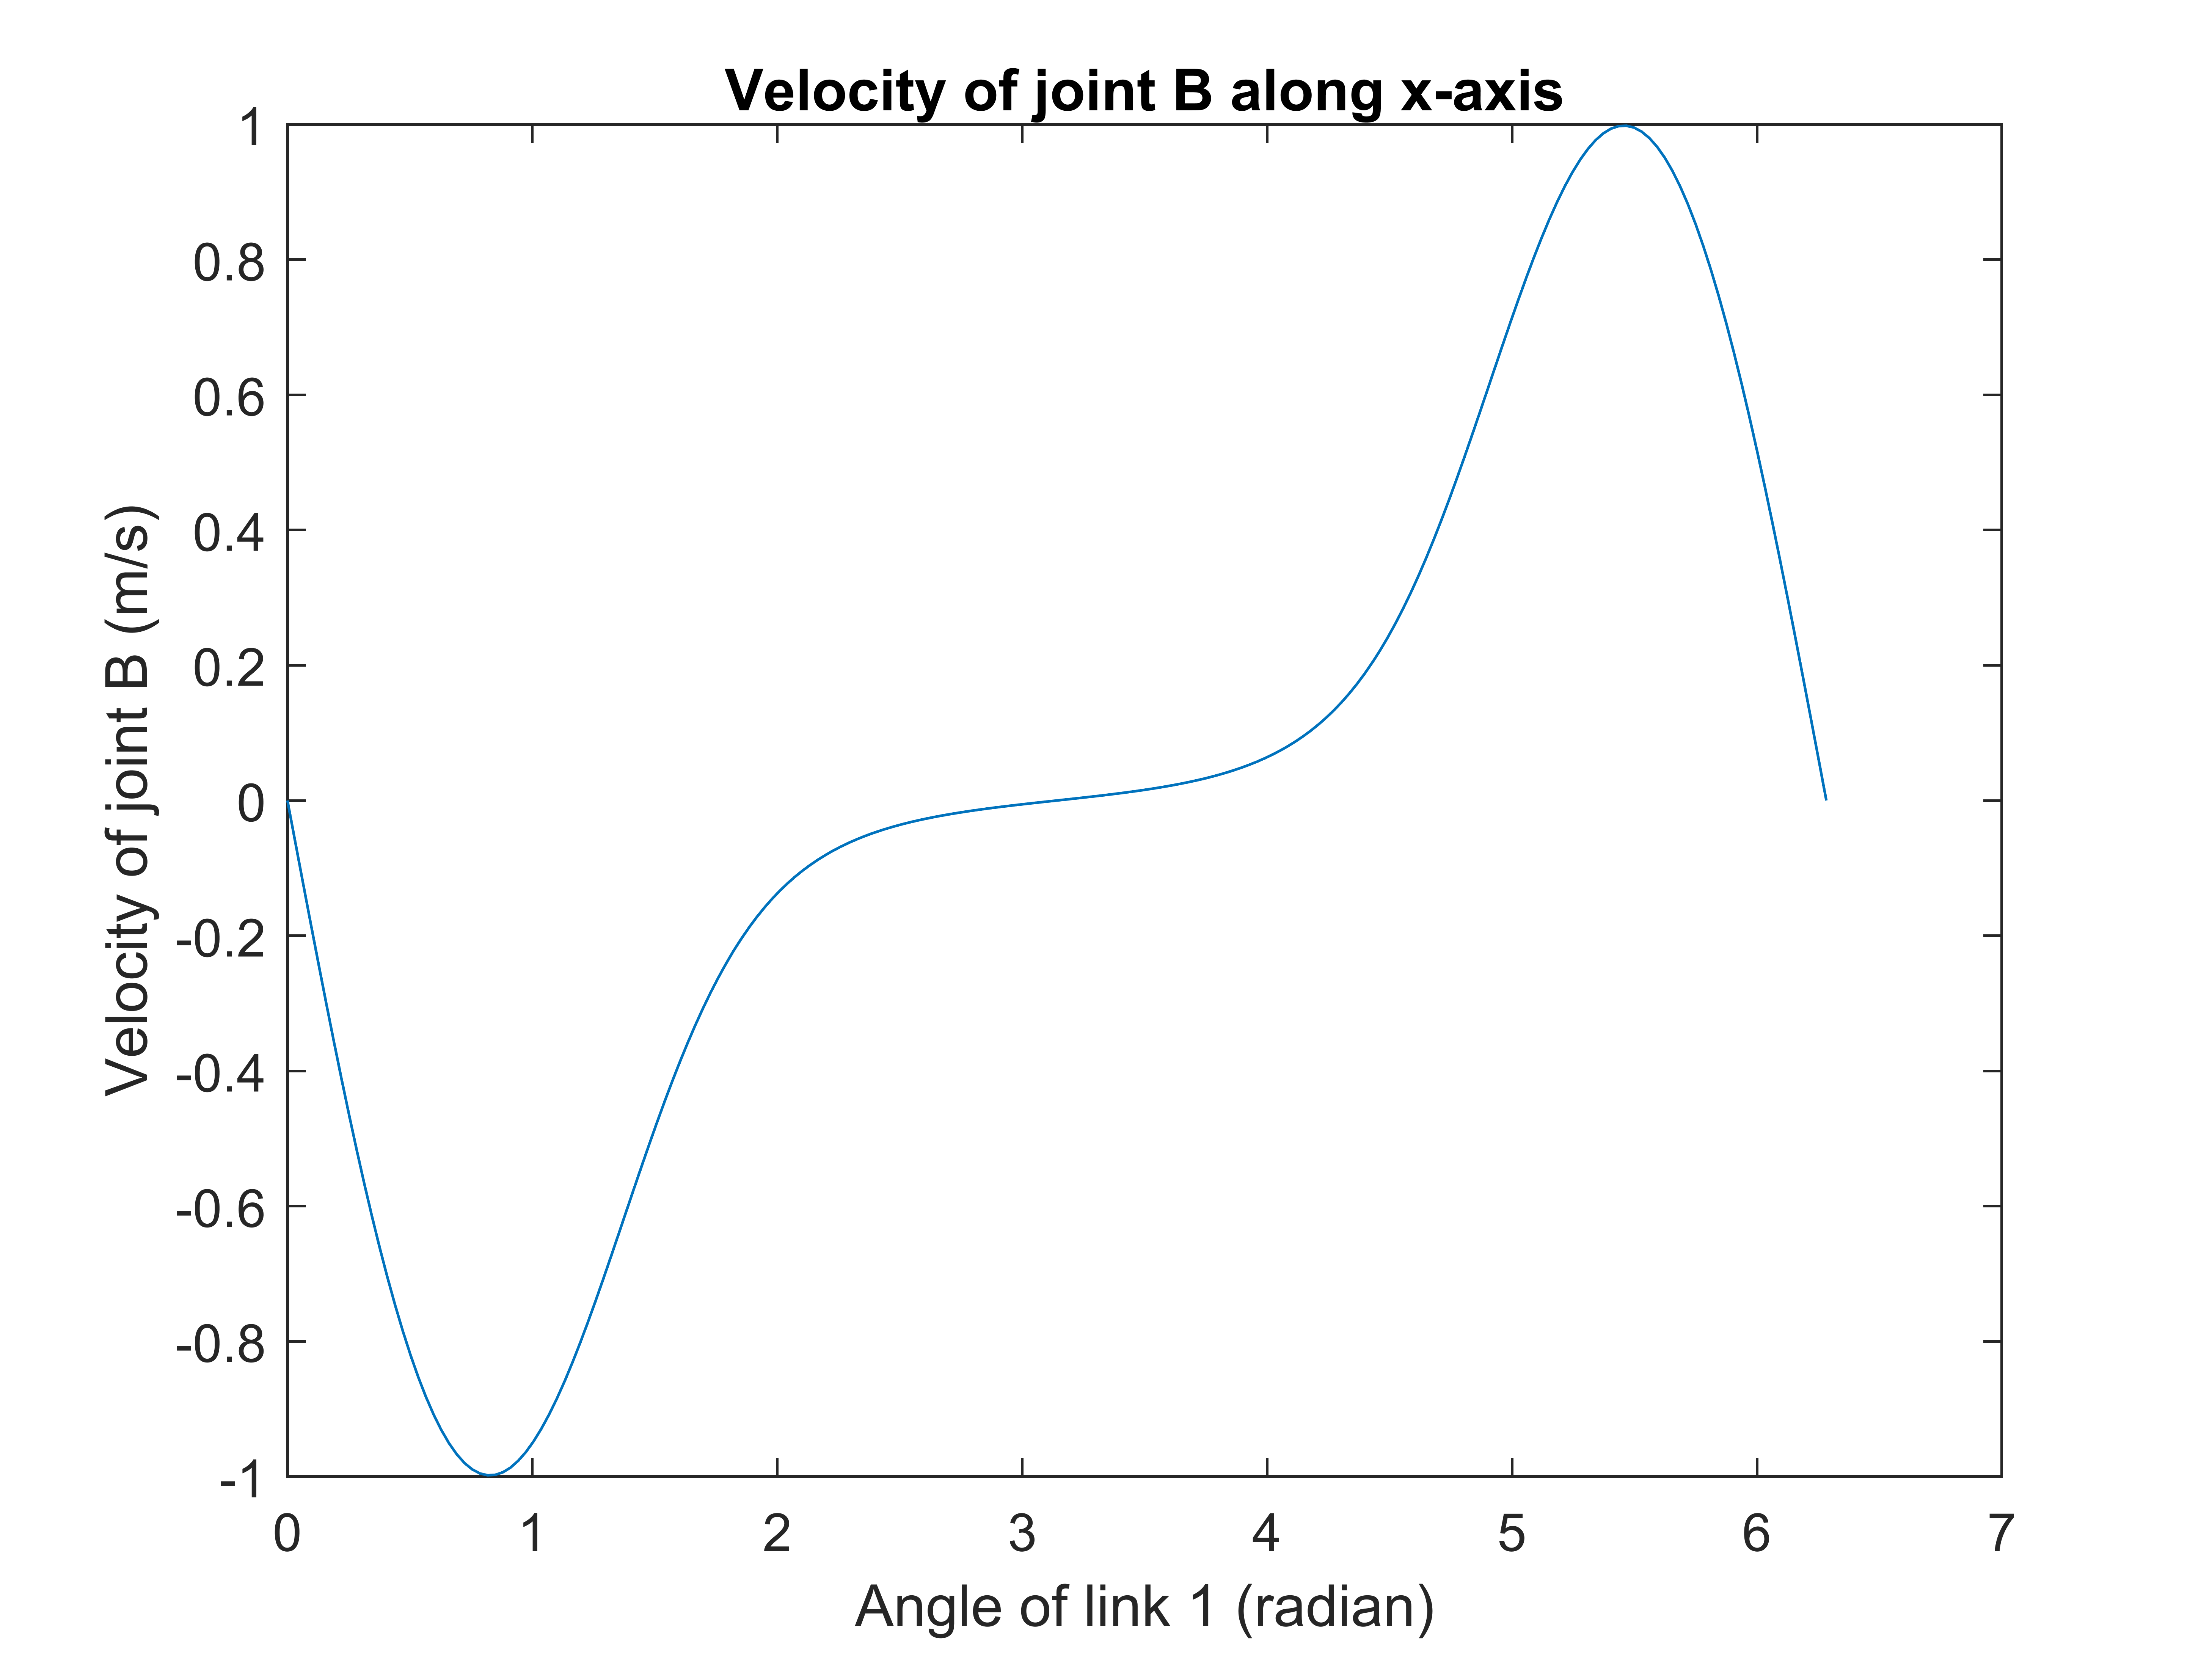
\includegraphics[width=60mm]{images/v_iRRRT.png}
	\end{figure}
\end{minipage}\hfill
\begin{minipage}{0.5\linewidth}
	\begin{figure}
		\centering
		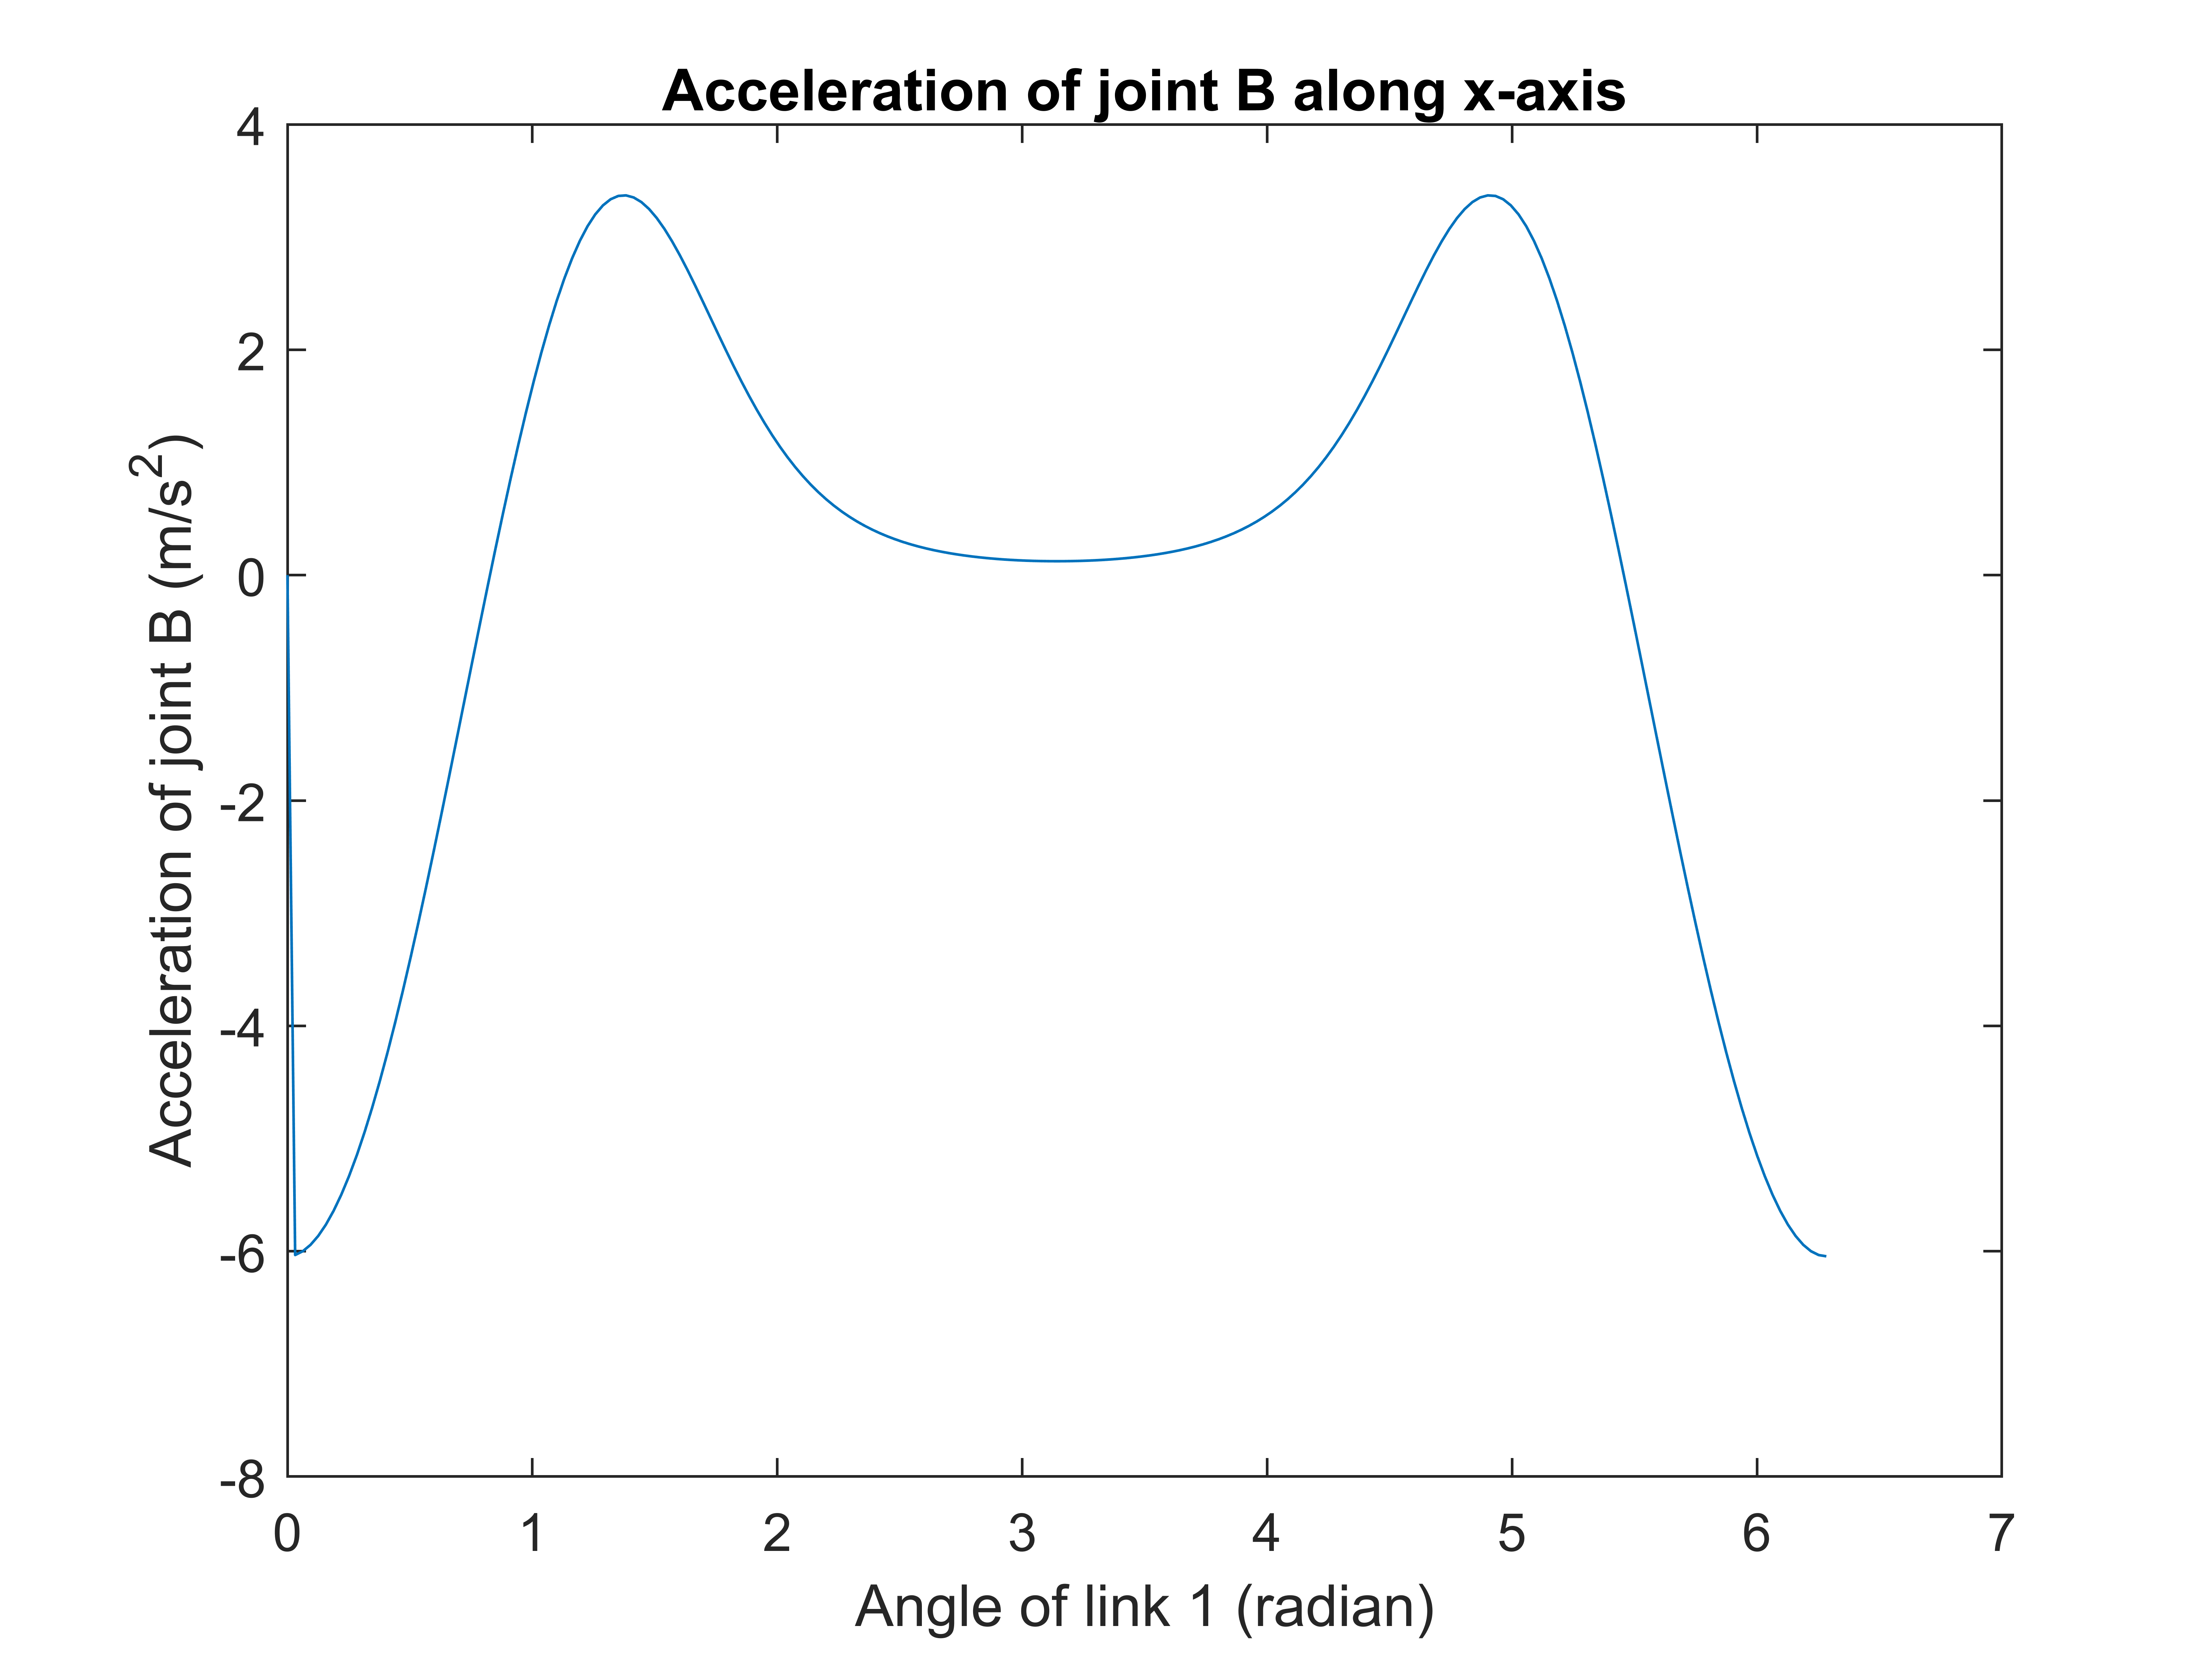
\includegraphics[width=60mm]{images/a_iRRRT.png}
	\end{figure}
\end{minipage}
\end{table}
\end{frame}